\documentclass{beamer}
\usepackage{lmodern}
\usepackage[utf8]{inputenc}
\usepackage{hyperref}
\usepackage{minted}
\usepackage{color}
\usepackage{booktabs}
\usepackage{tabularx}
\usepackage{array}
\usepackage{graphicx}

\setbeamertemplate{navigation symbols}{}
\mode<presentation>{\usetheme{Madrid}}

\title{Named Entity Classification}   
\author{Madita Huvar, Sanaz Safdel, Phillip R.-P.} 
\date{\today} 

\begin{document}



\begin{frame}
\titlepage
\end{frame} 

\begin{frame}
\frametitle{Inhaltsverzeichnis}
\tableofcontents
\end{frame} 


\section{Einführung}
\begin{frame}
	\frametitle{NER in der Forschung}
	Named Entity Recognition seit 1990er Jahren aktives Forschungsfeld. (Überblick: Borthwick, 1999, Tjong Kim Sang 2003, Marrero 2013)\\
	
	Grundlage für weitere Forschungsfelder im Bereich Information Retrieval, z.B. Semantic Annotation, Question Answering, Opinion Mining, usw. (Marrero 2013)
\end{frame}
\begin{frame}
	\frametitle{Was sind Named Entities}
	Named Entities sind Phrasen die Namen von Personen, Organisationen, Währungen, usw enthalten:\\
	\begin{exampleblock}{Beispiele für Named Entities}
		[ORG U.N. ], [PER Obama ], [MONEY Dollar], [LOC Moscow ] 
	\end{exampleblock}

\end{frame}
	\begin{frame}
		\frametitle{Unser Projekt}
		\begin{itemize}
			\item <+->Typischerweise werden Named Entity Recognition und Named Entity Classification (NEC) zusammen betrachtet.
			\item <+->Wenige Untersuchungen beschäftigen sich nur mit NEC. (Primadhanty 2014, He 2016, Spangler 2016)
			\item <+->Dieses Projekt konzentriert sich auf NEC und stellt die Frage, \textbf{welchen Einfluss Feature Selection auf die Klassifikationsergebnisse eines Named Entity Klassifizierers hat}.
			\item <+->Nutzung einfacher syntaktischer und lexikalischer Features, die in fast allen Forschungsarbeiten in ähnlicher Form genutzt wurden. \textit{(Toral, Munoz, 2006; Kazama, Torisawa, 2007; Ratinov, Roth 2009)} 
		\end{itemize}	

	\end{frame}
\section{Daten \& Tools}
	\subsection{Tools}
	\begin{frame}
			\frametitle{Tools}
			\begin{itemize}
				\item Python 3.4+
				\item Scikit Learn als Klassifizierer
				\item liac-arff
				\item matplotlib
				\item Weka zur Korpusanalyse
			\end{itemize}
	\end{frame}
	\subsection{Korpus}
	\begin{frame}
			\frametitle{Korpus}
			\begin{itemize}
				\item Für Named Entity Klassifikation wird OntoNotes Korpus 2012 genutzt. \textit{(OntoNotes Release 5.0 2012)}
				\item Englischen Nachrichtentexte des 'The Wall Street Journal'.
				Für die Entwicklungsphase bereits vorgefertigtes Developmenttest.
				\item Für die Klassifikation der Named Entities werden die bereits vorgefertigten Trainings- und Testdatensets genutzt.
			\end{itemize}
			 \begin{table}
			 	\caption{Anzahl an atomaren Named Entities}
			 	\begin{tabular}{ccc}
			 		\toprule
					Developmentset & Trainingset & Testset\\
			 		\midrule
					3325 & 23686 & 2996\\
			 		\bottomrule
			 	\end{tabular}
			 	\label{tab:datasets}
			 \end{table}
	\end{frame}
		\begin{frame}
			\frametitle{Korpusreader}
			\begin{itemize}
				\item Für Extraktion der Named Entities wurde ein Korpusreader erstellt.
				\item 	Der Reader extrahiert alle Named Entities, inklusive POS-Tags der einzelnen Token, Phrasenart, Kontextwörtern (ne-1, ne+1), und ordnet ihnen Klassen zu.
			\end{itemize}
			
			
		
			
			\begin{exampleblock}{Extrahierte Instanz der Korpusreader-Klasse}
				\{'PERSON':[['Peter', 'NNP'],['Mokaba', 'NNP'],'NP', ('Says', ',')]\}
			\end{exampleblock}
			
		\end{frame}
	
	\subsection{Korpusklassen}
		\begin{frame}
			\frametitle{Korpusklassenbalancierung}
				\begin{table}
				\caption{Klassen im OntoNotes Korpus \textit{(OntoNotes Release 5.0 2012)}}
				\begin{tabularx}{\textwidth}{Xc}
					\toprule
					Klassen  & Trainingset \\
					\midrule
					ORG  & 5788 \\
					DATE & 4080  \\
					PERSON & 3756 \\
					GPE & 3601 \\
					CARDINAL & 1852 \\
					MONEY & 1509  \\
					NORP & 1484 \\
					PERCENT & 1061  \\
					FAC, LOC, PRODUCT, EVENT, WORK\_OF\_ART, LAW, LANGUAGE, TIME, QUANTITY, ORDINAL & $<$ 1800 \\
					\bottomrule
				\end{tabularx}
				\label{tab:datasets}
			\end{table}
		\end{frame}
			\begin{frame}
				\frametitle{Verteilung Korpusklassen}
				\begin{itemize}
					\item Zehn Klassen enthalten nur wenige NE-Instanzen. Diese werden aus dem balancierten Korpus entfernt.
					\item Semantisch ähnliche Klassen NORP und GPE werden zusammengefasst.
					\item Numerische Klassen MONEY, PERCENT und CARDINAl werden ebenfalls zusammengefasst.
				\end{itemize}
			\end{frame}
	\begin{frame}
		\frametitle{Beschreibung neuer Korpusklassen}
		\begin{table}
			\caption{Balancierte Klassen}
			\begin{tabularx}{\textwidth}{lX}
				\toprule
				Klassen  & Beschreibung \\
				\midrule
				PERSON 	& People, including fictional \\
				NORP\_GPE &	Nationalities or religious or political groups
				Countries, cities, states\\
				ORGANIZATION &	Companies, agencies, institutions, etc.\\
				DATE &	Absolute or relative dates or periods\\
				PERCENT\_MONEY\_CARDINAL &	Percentage (including “\%”)
				Monetary values, including unit
				Numerals that do not fall under another type \\
				\bottomrule
			\end{tabularx}
			\label{tab:datasets}
		\end{table}
	\end{frame}

	\begin{frame}
			\frametitle{Verteilung Korpusklassen}
			 \begin{table}
			 	\caption{Verteilung der Klassen nach Balancierung}
			 	\begin{tabular}{lccc}
			 		\toprule
			 		Klassen  & Developmentset & Trainingset & Testset \\
			 		\midrule
			 		ORG  & 930 & 5857 & 859 \\
			 		GPE\_NORP & 732 & 5134 & 588 \\
			 		PERCENT\_CARDINAL\_MONEY & 564 & 4672 & 529 \\
			 		DATE & 613 & 4254 & 601 \\	 		
			 		PERSON & 486 & 3759 & 413 \\
			 		\bottomrule
			 	\end{tabular}
			 	\label{tab:datasets}
			 \end{table}
	\end{frame}


\section{Klassifizierer}
	\begin{frame}
		\frametitle{Beispielinstanz}
		\begin{exampleblock}{Beispielinstanz zur Veranschaulichung der Features}
		[ ['North', 'NNP'],['-', HYPH], ['America', 'NNP'], 'NP', (',', 'and')]
	\end{exampleblock}
		
	\end{frame}
	\subsection{Features für den Baseline-Klassifizierer}
	\begin{frame}
		\frametitle{Features für den Baseline-Klassifizierer}
		Anzahl der Features: 1317
					 \begin{table}
					 	\caption{Features für den Baseline-Klassifizierer}
					 	\begin{tabularx}{\textwidth}{llX}
					 		\toprule
							Feature & Wert & Beschreibung\\
					 		\midrule
					 		Unigram & numerisch & Vorkommen der Unigramme, die mindestens fünfmal im Trainingscorpus vorkommen. \textit{(Mayfield 2003)} \\
					 		\bottomrule
					 	\end{tabularx}
					 	\label{tab:baselinef}
					 \end{table}
	\end{frame}
	\subsection{Erweitertes Featureset}
	\begin{frame}
		\frametitle{Erweitertes Featureset I}
		Anzahl der Features: 1716
 			\begin{table}
 				\caption{Features für den Klassifizierer I}
 				\begin{tabularx}{\textwidth}{llX}
 					\toprule
 					Feature & Wert & Beschreibung\\
 					\midrule
 					Unigram & numerisch & Vorkommen der Unigramme (lemmatisiert), die mindestens fünfmal im Trainingscorpus vorkommen. \textit{(Mayfield 2003)} \color{red}(america : 1, north : 1)\\
 					POS & numerisch  & Häufigkeit von 36 POS-Tags aus der Penn Treebank \textit{(Florian, Chieu 2003)} \color{red}NNP: '2'\\
 					isAllCaps & boolean & Wörter nur in Großschreibung \textit{(Nadeau 2006)} \color{red} (0)\\
 					Context & numerisch & Vorkommen der Kontexttokens. Beinhaltet Vorgänger- und Nachfolgetoken der NE. \textit{(Munro 2003)}  \color{red} (,\_and : 1)\\
 					containsDigit & boolean & Vorkommen von Nummern. \color{red} (0)\textit{}\\
 					\bottomrule
 				\end{tabularx}
 				\label{tab:allf1}
 			\end{table}
 	\end{frame}
 		\begin{frame}
 			\frametitle{Erweitertes Featureset II}
 					\begin{table}
 						\caption{Features für den  Klassifizierer II}
 						\begin{tabularx}{\textwidth}{llX}
 							\toprule
 							Feature & Wert & Beschreibung (Beispielwert)\\
 							\midrule
 							isInWiki & boolean & Vorkommen der NE in der Wikipedia. \textit{(Toral, Munoz 2006)} \color{red} (1)\\
 							isTitle & boolean & Prüft, ob Titelbezeichnungen (z.B. Mr. MA) vorkommen. \textit{(Ratinov, Roth 2009)} (0)\\
 							isNP & boolean & Ist NE eine Nominalphrase. \textit{(Sánchez, Cuadrado 2009)} \color{red} (1)\\
 							isName & boolean & Prüft, ob Vornamen vorkommen.\textit{(Ratinov, Roth 2009)} (0)\\
 							containsDash & boolean & Vorkommen von Viertelgeviertstrichen. \textit{(Mayfield 2003)} (1) \\
 							isComName & boolean & Prüft aus kommerzielle Bezeichner \color{red} (0)\\
 							\bottomrule
 						\end{tabularx}
 						\label{tab:allf2}
 					\end{table}
 		\end{frame}
	\subsection{Klassifizierertyp}
	\begin{frame}
		\frametitle{Klassifizierertyp}
		\begin{itemize}
			\item<+->Zur Klassifizierung der NE wird eine Support Vector Maschine mit linearem Kernel verwendet.
			\item<+-> SVM (sklearn.svm.LinearSVC)\\
						
			Featurevektoren haben sehr viele Features
			daher linearer Kernel.\\
			Mapping in höheren Featurespace eines nicht-linearen Kernels bringt kaum Klassifizierungsverbesserungen. \textit{(Chih-Wei Hsu 2003)}
			\item<+->\textit{Alternativ wurde ein Decisiontree getestet, dieser hatte allerdings mit allen Featurekombinationen tendenziell schlechtere Evaluationsergebnisse. Zudem trainiert der SVM deutlich schneller.}
		\end{itemize}
	\end{frame}

	\subsection{Erfahrungen mit den Korpusklassen}
	\begin{frame}
		\frametitle{Erfahrungen mit den Korpusklassen I}
		Wie die ROC-Kurve zeigt, hat der Klassifizierer insbesondere Schwierigkeiten, die Klassen PERSON und ORG und GPE\_NORP zu unterscheiden.\\
	\end{frame}
	\begin{frame}
		\frametitle{ROC Curve}
		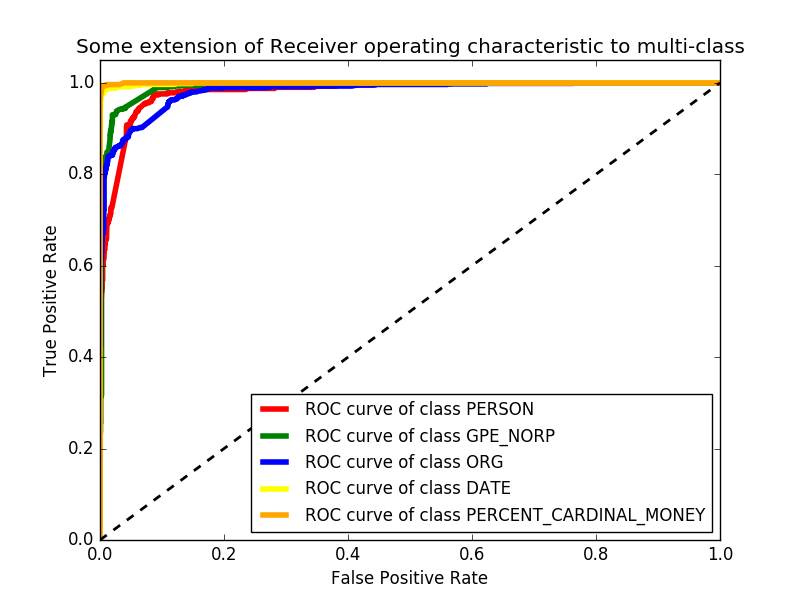
\includegraphics[scale=0.54]{roc_curve.png}
	\end{frame}
		\begin{frame}
			\frametitle{Erfahrungen mit den Korpusklassen II}
			\begin{table}
				\caption{Confusion Matrix}
				\begin{tabularx}{\textwidth}{llllll}
					\toprule
					361 & 28 & 22 & 2 & 0 & PERSON\\
					29 & 549 & 10 & 0 & 0 & GPE\_NORP\\
					71 & 45 & 736 & 6 & 1 & ORG\\
					0 & 2 & 1 & 591 & 7 & DATE\\
					0 & 2 & 0 & 2 & 525 & PERCENT\_CARDINAL\_MONEY\\
					\bottomrule
				\end{tabularx}
				\label{tab:allf2}
			\end{table}			
		\end{frame}
	\begin{frame}
		\frametitle{Beobachtungen zur Confusion-Matrix}
		\begin{itemize}
			\item Von 361 PERSON Entities, werden 71 als ORG und 29 als GPE\_NORP klassifiziert.

			\item Numerische Klassen und Datum werden fast zu 100\% erkannt.
		\end{itemize}
	\end{frame}	
\section{Evaluation}
	\begin{frame}
		\frametitle{Featureselektion I}
		\begin{itemize}
			\item <+->Insgesamt wurden elf Features eingesetzt.\\
			
			\item <+->Um die Performance der einzelnen Features zu testen, wurde die Potenzmenge des Featuresets gebildet.\\
			
			\item <+->Schließlich wurde der Klassifizierer auf allen 1013 Teilmengen durchgeführt.\\
		\end{itemize}
		
	\end{frame}
	\begin{frame}
		\frametitle{Featureselektion II}
			Für die Evaluation entscheidend waren alle Teilmengen, die die Features 'Unigram' und 'Context' enthalten und mind. drei Features 3 besitzen.\\
					
			\begin{itemize}
				\item Accuracy aller Teilnmengen ohne diese Features: \textless 69 \%.
				\item Accuracy nur mit Unigram und Context: 87.42\%
			\end{itemize}

					
	\end{frame}
		\begin{frame}
			\frametitle{Featureselektion III}
			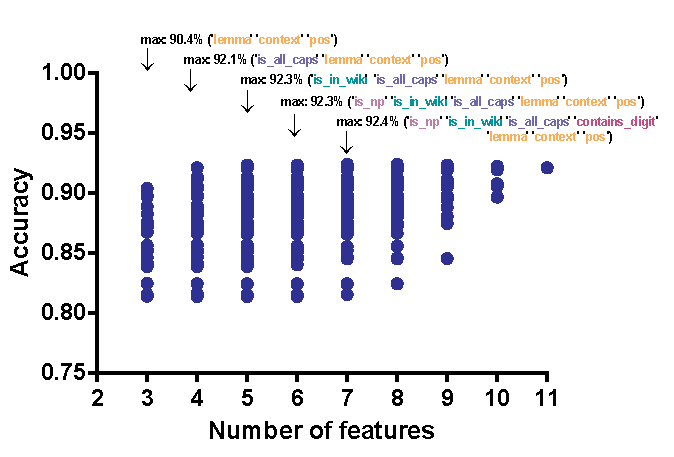
\includegraphics[scale=0.9]{accuracy.pdf}\\

		\end{frame}
	\begin{frame}
		\begin{itemize}
			\frametitle{Featureselektion IV}
			\item <+->Beste Features: 'Unigram', 'Context'\\
			\item <+->Höchste Accuracy: Ab sieben Features. Ab vier Features kaum mehr Verbesserung der Accuracy \\
			\item <+->Features, die zur Erhöhung der Accuracy beitragen: 'POS', 'is\_all\_caps', 'is\_in\_wiki', 'is\_np', 'contains\_digit'\\
			\item <+->Das Featureset aus vier Features: 'Unigram', 'Context', 'POS', 'is\_all\_caps' erreicht die beste Accuracy bei möglichts kleinem Featureset.
		\end{itemize}
	\end{frame}
	\begin{frame}
		\frametitle{Evaluation}
		Evaluationsergebnisse der Baseline im Vergleich mit optimalen Testset
				\begin{table}
					\caption{Final Evaluation}
					\begin{tabularx}{\textwidth}{llll}
						Featureset & & Accuracy\\
						\toprule
						Baseline & unbalanced & 0.7867578489285\\
								 & balanced & 0.840802675585\\
						Optimales Featureset	 & unbalanced & 0.87286291576\\
								 & balanced & 0.923745819398\\
						\bottomrule
					\end{tabularx}
					\label{tab:allf2}
				\end{table}	
		
		
		
		
	\end{frame}
		\subsection{Probleme}
		\begin{frame}
			\frametitle{Probleme}
			Context bezieht auch Satzzeichen ein (oft ',' oder '.'), dies könnte man auf alphanumerische Strings beschränken.\\
			
			Klassifikationsfehler im Testset, da nur die automatisch annotierte Testsetversion von OntoNotes v5 zur Verfügung steht.\\
			
			\begin{exampleblock}{Beispiel für falsch klassifizierte Instanz}
				\{'ORG': [['American', 'JJ'], 'NP', ('to', 'notions')]\}\\classified as ['GPE\_NORP']
			\end{exampleblock}
			
			
		\end{frame}
\section{Ausblick}
	\begin{frame}
		\frametitle{Ausblick}
		
	\end{frame}
\section{Referenzen}
	\begin{frame}
		\frametitle{Referenzen}
		\begin{itemize}
			\item Cho, H.; Okazaki, N. (2013): Named entity recognition with multiple segment representations. In: Information Processing \& Management 49\\
			\item Derczynski, L.; Maynard, D.; Rizzo, G.; van Erp, M. (2015): Analysis of named entity recognition and linking for tweets. In: Information Processing \& Management 51 (2), S. 32–49.\\
			\item Konkol, M.; Brychcín, T.; Konopík, M. (2015): Latent semantics in Named Entity Recognition. In: Expert Systems with Applications 42 (7), S. 3470–3479.\\
			\item Agerri, R.; Rigau, G. (2016): Robust multilingual Named Entity Recognition with shallow semi-supervised features. In: Artificial Intelligence 238, S. 63–82.\\
			\item Tjong Kim Sang,E.; De Meulder, F. (2003): Language-Independent Named Entity Recognition.\\
		\end{itemize}
	\end{frame}
	\begin{frame}
		\begin{itemize}
			\item Marrero, M.; Urbano, J. (2013): Named Entity Recognition. Fallacies, challenges and opportunities. In: Computer Standards \& Interfaces 35 (5), S. 482–489.\\
			\item Mayfield, J.; McNamee, P. (2003): Named entity recognition using hundreds of thousands of features. In: Walter Daelemans und Miles Osborne (Hg.): Proceedings of the seventh conference on Natural language learning at HLT-NAACL 2003 -. the seventh conference. Edmonton, Canada. Morristown, NJ, USA: Association for Computational Linguistics, S. 184–187.\\
			\item Marrero, M.; Sánchez-Cuadrado, S. (2009): Evaluation of Named Entity Extraction Systems.\\
			\item Weischedel, R. (2013): OntoNotes release 5.0. [Philadelphia, Pa.]: Linguistic Data Consortium.\\
			\item Nadeau, D.; Turney, P. (2006): Unsupervised Named-Entity Recognition: Generating Gazetteers and Resolving Ambiguity. Berlin.
		\end{itemize}
	\end{frame}
	\begin{frame}
			\begin{itemize}
				\item Radu F.; Abe It. (2003):  Named Entity Recognition
				through Classifier Combination. In
				Proceedings of 	CoNLL-2003.
				\item Chieu H. (2003): Named Entity Recognition with a Maximum Entropy Approach. In Proceedings of CoNLL-2003.
				\item Borthwick, A. (1999): A
				Maximum Entropy Approach to Named Entity Recognition, Diss., New York.\\
				\item Primadhanty, A.; Carreras, X. (2014): Low-Rank Regularization for Sparse Conjunctive Feature Spaces:
				An Application to Named Entity Classification. In Proceedings of the 53rd Annual Meeting of the Association for Computational Linguistics.
				\item He, Q.; Spangler, S. (2016): Semi-supervised data integration model for named entity classification. Google Patents.
			\end{itemize}
	\end{frame}
	\begin{frame}
			\begin{itemize}
				\item Munro, R.; Ler, D. (2003): Meta-Learning Orthographic and Contextual Models for Language Independent Named Entity Recognition. In Proceeding
				CONLL '03 Proceedings of the seventh conference on Natural language learning at HLT-NAACL.\\
				\item Ratinov, L.; Roth, D. (2009): Design Challenges and Misconceptions in Named Entity Recognition. In Proceedings of the Thirteenth Conference on Computational Natural Language Learning (CoNLL).
				Toral, Antonio; Munoz, Rafael (2006): A proposal to automatically build and maintain gazetteers for Named Entity Recognition by using Wikipedia.
			\end{itemize}
	\end{frame}

\end{document}
